\documentclass{icmmcm}
%\usepackage[dvips]{graphicx}  % For importing graphics for use with
                              % dvips.
\usepackage[pdftex]{graphics} % For importing graphics for use with
                              % pdftex or pdflatex.
\usepackage[numbers]{natbib}

%%% Sample ICM/MCM Contest Submission
%%%
%%% C.M. Connelly <cmc@math.hmc.edu>
%%%   for the Department of Mathematics, Harvey Mudd College
%%%   Copyright 2003. 


%%% ---------------
%%% Local Command and Environment Definitions

%%% If you have any local command or environment definitions, put them
%%% here or in a separate style file that you load with \usepackage.

% \newtheorem declarations
\newtheorem{Theo1}{Theorem}
\newtheorem{Theo2}{Theorem}[section]
\newtheorem{Lemma}[Theo2]{Lemma}
% Each of the above defines a new theorem environment.
% Multiple theorems can be done in the same environment.
% Theo2's number is defined by the subsection it's in.
% Theo3 uses the same numbering counter and numbering system as
% Theo2 (that's the meaning of [Theo2]).


%%% TeX has an excellent hyphenation algorithm, but sometimes it
%%% gets confused and needs some help.
%%%
%%% For words that only occur once or twice, you can insert hints
%%% directly into your text, as in
%%%
%%%    our data\-base system is one of the most complex ever devised
%%%
%%% For words that you use a lot, and that seem to keep ending up at
%%% the end of a line, however, inserting the hints each time gets to
%%% be a drag.  You can use the \hyphenation command  to globally tell
%%% TeX where to hyphenate words it can't figure out on its own.

\hyphenation{white-space}

%%% End Local Command and Environment Definitions
%%% ---------------


%%% ---------------
%%% Title Block

\title{Conspirators Investigation}

%%% Which contest are you taking part in?  (Just one!)

\contest{ICM}

%%% The question you answered.  (Again, just the one.)

\question{C}

%%% Your Contest Team Control Number
\team{15118}


%%% A normal document would specify the author's name (and possibly
%%% their affiliation or other information) in an \author command.
%%% Because the ICM/MCM Contest rules specify that the names of the
%%% team members, their advisor, and their institution should not
%%% appear anywhere in the report, do *not* define an \author command.

%%% Defining the \date command is optional.  If you leave it blank,
%%% your document will include the date that the file is typeset, in
%%% the form  ``Month dd, yyyy''.

% \date{}

%%% End Title Block
%%% ---------------

\begin{document}

%%% ---------------
%%% Summary

\begin{summary}
  The contest rules specify that you should include a one-page summary
  of your report.  This page appears before the rest of the report,
  and will have a special header attached to it that takes up the top
  2.5" of the page.

  By typing your summary inside a \texttt{summary} environment, \TeX\ will
  handle the formatting of that page correctly, including leaving
  space at the top of the page and not numbering the page.
  
  It will also reset the page numbers so that the first page of your
  report is labeled correctly.
  
  What should you put here?  Basically, you want a brief restatement
  of the problem followed by a largely \emph{non-technical}
  description of what you've done.  Try to avoid using mathematical
  notation.
  
  You probably want to write a few paragraphs, around half to
  two-thirds of a page.

  For 2009, the COMAP folks said the following about the summary:
  \begin{quotation}
    The summary is a very important part of your MCM paper. The
    judges place considerable weight on the summary, and winning
    papers are sometimes distinguished from other papers based on
    the quality of the summary. To write a good summary, imagine
    that a reader may choose whether to read the body of the paper
    based on your summary. Thus, a summary should clearly describe
    your approach to the problem and, most prominently, what your
    most important conclusions were. The summary should inspire a
    reader to learn the details of your work.  Your concise
    presentation of the summary should inspire a reader to learn
    the details of your work. Summaries that are mere restatements
    of the contest problem, or are a cut-and-paste boilerplate
    from the Introduction are generally considered to be
    weak.

To Summarize:
\begin{description}
\item[Restatement Clarification of the Problem]
---

\item[Assumptions with Rationale/Justification]---emphasize those
  assumptions that bear on the problem. List clearly all variables
  used in your model.

\item[Model Design and justification for type model used/developed.]

\item[Model Testing and Sensitivity Analysis, including error
  analysis, etc.]

\item[Discuss strengths and weakness to your model or approach.]

\item[Provide algorithms] in words, figures, or flow charts (as a step
  by step algorithmic approach) for all computer codes developed.
\end{description}
 \citep{comap-mcm-rules}
\end{quotation}

\end{summary}
 
%%% End Summary
%%% ---------------

%%% ---------------
%%% Print Title Block, Contents, et al.

\maketitle
\tableofcontents

%%% Uncomment the following lines by deleting the % sign
%%% if you have figures or tables in your report:
\listoffigures
\listoftables  
 
%%% End Print Title Block, Contents, et al.
%%% ---------------

\section{Introduction}%
\label{sec:introduction}


Our organization, the Intergalactic Crime Modelers (ICM) is working
for a criminal case of a bank company.  There are indications that  there is a conspiracy within the company.  
It is believed that the conspirators want to embezzle funds from the company and to steal funds from credit card 
Careful logs have been kept of whom has sent messages related to each topic and whom received these messages.
... [explain the scenario and what we are trying to solve]

The goal to approach this problem is to determine a priority list, 
to draw a discriminate line, and if possible to find
conspiracy leaders. In addition, we also want to use semantic
network analysis to improve the result and examine applications of
our developed techniques in other fields such as diseased biology.
[TODO: Explain more.]

\noindent -------------------- TODO:
the history and context of the problem,
and your work and results.  Your introduction should be more detailed
and technical than your summary.  You may also want to include an
outline of your report, along the lines of
\begin{quotation}
  In Section~1 we give our definitions and notation. Section~2
  describes our numerical experiments\ldots{}..
  
  We prove our main result, Theorem~6, in Section~5\ldots{}.
\end{quotation}
Of course you would replace the numbers in that example with
appropriate \verb|\ref| commands pointing to the correct
\verb|\label|s in your source.\\
-----------------------

\section{Given Information}
\begin{enumerate}
\item We are given that Jean, Alex, Elsie, Paul, Ulf, Yao,
and Harvey are conspirators.
\item We are given that Darlene, Tran, Jia, Ellin, Gard, Chris,
Paige, and Este are \textit{not} conspirators.
\item There are 83 nodes, 400 links, and 15 considered topics.
\item Topics 7, 11, and 13 are known to be suspicious topics.
\end{enumerate}

\section{Assumptions}

\begin{enumerate}
\item Assume that it is unlikely that conspirators communicate
conspiratorial topics to non-conspirators.

\item Assume that the conspirators are discussing the suspicious topic.

\item Assume that the more that a person discusses a suspicious topic the more likely that person is to be a conspirator.  
%\item Assume that the more involved a person is in a topic, the m
\item Assume that non-conspirators are not likely to be participating in discussions of 

\item Assume that conspirators are more likely to be discussing topics that relate to the conspiracy than anyone else.
Therefore if a know conspirator is participating a lot in a conversation topic,
the topic is more likely to be related to the conspiracy than not. 
\end{enumerate}
\section{Model Design}

\subsection{Setup}
\begin{enumerate}
\item For each person $i$, $0\leq i\leq 82$, we define three parameters: 

\quad (1) the probability (``certainty'')
that each person is a conspirator, $c_i,$
where $0\leq c_i \leq 1.$ 
We first set $c_i = 0$ for those

\quad (2) 

\item We use python to model the problem.
\end{enumerate}
\subsection{Theorems}
\begin{Theo1}
For a given point $C$, of all the paths from point $A$ to point $B$, the number of repeaters needed at point $C$ is equivalently increased by 
$$\frac{\text{nPaths}(A,C)\cdot \text{nPaths}(C,B)}{\text{nPaths}(A,B)},$$
where $\text{nPaths}(X,Y)$ is a function that returns the number of possible \emph{shortest} paths from $X$ to $Y$, which is given in Theorem 2.
\end{Theo1}
{\bf Proof.}
It follows from the principle of counting:
\begin{align*} \text{The weight for additional repeaters at C}
&=\frac{\text{The number of paths from A to B via C}}{\text{The number of paths from A to B}}\\
&=\frac{\text{nPaths}(A,C)\cdot \text{nPaths}(C,B)}{\text{nPaths}(A,B)}.
\end{align*}\hfill $\Box$

{\bf Proof.}
There are six triangle subsectors of a hexagon. For each sector, the number of triangle is $1, 3, 5, \ldots, (2n-1)$. Each sector represents one area. Thus, the total number of areas is
$$6(1+ 3+ 5+\cdots+ (2n-1))=6n^2.$$\hfill $\Box$

%%=================NEW SECTION
\section{Model Testing}

Take a look at an example below, where we put the city into our hexagonal coordinate (Both X and Y range from -3 to 3):
\begin{table}[htbp]
  \begin{center}
    \begin{tabular}{@{}c|rrrrrrr@{}} \toprule
X and Y  	&-3 	&-2 		&-1		&0		&1		&2		&3\\ \midrule   
3&15.53	&34.87	&36.03	&32.00	&0.00	&0.00	&0.00    \\ 
2&36.73	&76.12	&104.57	&81.22	&43.00	&0.00	&0.00	\\
1&37.13	&94.27	&137.75	&138.05	&91.57	&54.00	&0.00	\\
0&31.0	&82.1	&134.47	&\textbf{158.42}	&140.13	&83.07	&35.00	\\
-1&0.00	&51.0	&113.25	&137.35	&145.05	&111.92	&39.12	\\
-2&0.00	&0.00	&49.00	&89.37	&99.00	&92.42	&46.47	\\
-3&0.00	&0.00	&0.00	&33.00	&32.15	&36.18	&27.72	\\
 \bottomrule	
    \end{tabular}
  \end{center}
  \caption[A Distribution of Repeaters for a Uniform Distribution of People]{The table of the number of conversations (reflecting the number of repeaters) at each point. The number of people is 1000. The level of hexagons is 3.}
  \label{tab:uniform}
\end{table}

From Table~\ref{tab:uniform}, we have the total number of repeaters of 2,780. Hence, the actual number of repeaters needed (with help of PL tones) is 51.48. As there are $6\times(3^2)=54$ regions as well, the number of repeaters needed per 1 PL tone per 1 location is 0.953. This can be done easily since we have 3 frequency sets to serve. One concern is the service at the peak: the middle (point $(0,0)$). The original number of repeaters needed is 158.42. By using PL tones, we have the avearge of $2.93$ users using one PL tone. Again, this use can be accommadated by 3 different sets of frequencies. Thus, in this case, the total number of repeaters required is 51.48, approximately \boxed{52 \text{ repeaters}} , each holding differnt 54 PL tones.

%Figure~\ref{sample1} is an example of repeater coordination.
%\begin{figure}[!hbtp]
%\makebox[\textwidth]{\framebox[8cm]{\rule{0pt}{8cm}}}
%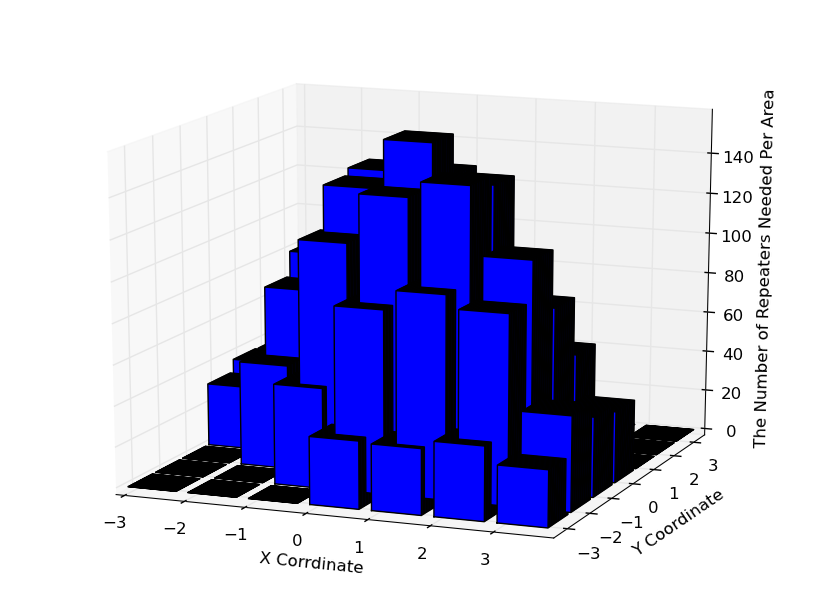
\includegraphics[width=7cm]{sample1.png}
%\caption{Sample 1 Distribution of Repeaters (Maximum at the Middle).\label{white}}
%\end{figure}

Figure~\ref{fig:sample1} is an example of repeater coordination.
\begin{figure}[ht]
\begin{center}
\scalebox{0.6}{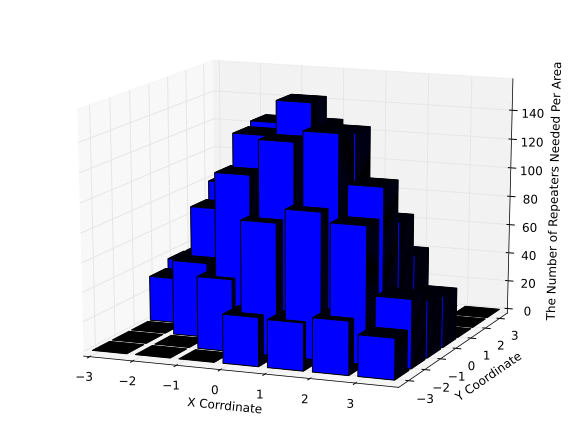
\includegraphics{sample1}}
\end{center}
\caption[A Distribution of Repeaters for a Uniform People Distribution]{A Distribution of Repeaters (Maximum at the Middle).\label{sample1}}%
\label{fig:sample1}
\end{figure}

\section{Sensitivity Analysis And Error Analysis}
We do several cases and find the standard deviation. Also, we can try to plot a function of the minimum number of repeaters depending on the number of people. If we were to plot this graph, there would be a limit point in which no repeater coordination can serve that number of simultaneous users.

Figure~\ref{sensitivity} represents the data test for sensitivity.
\begin{figure}[ht]
\begin{center}
\scalebox{0.6}{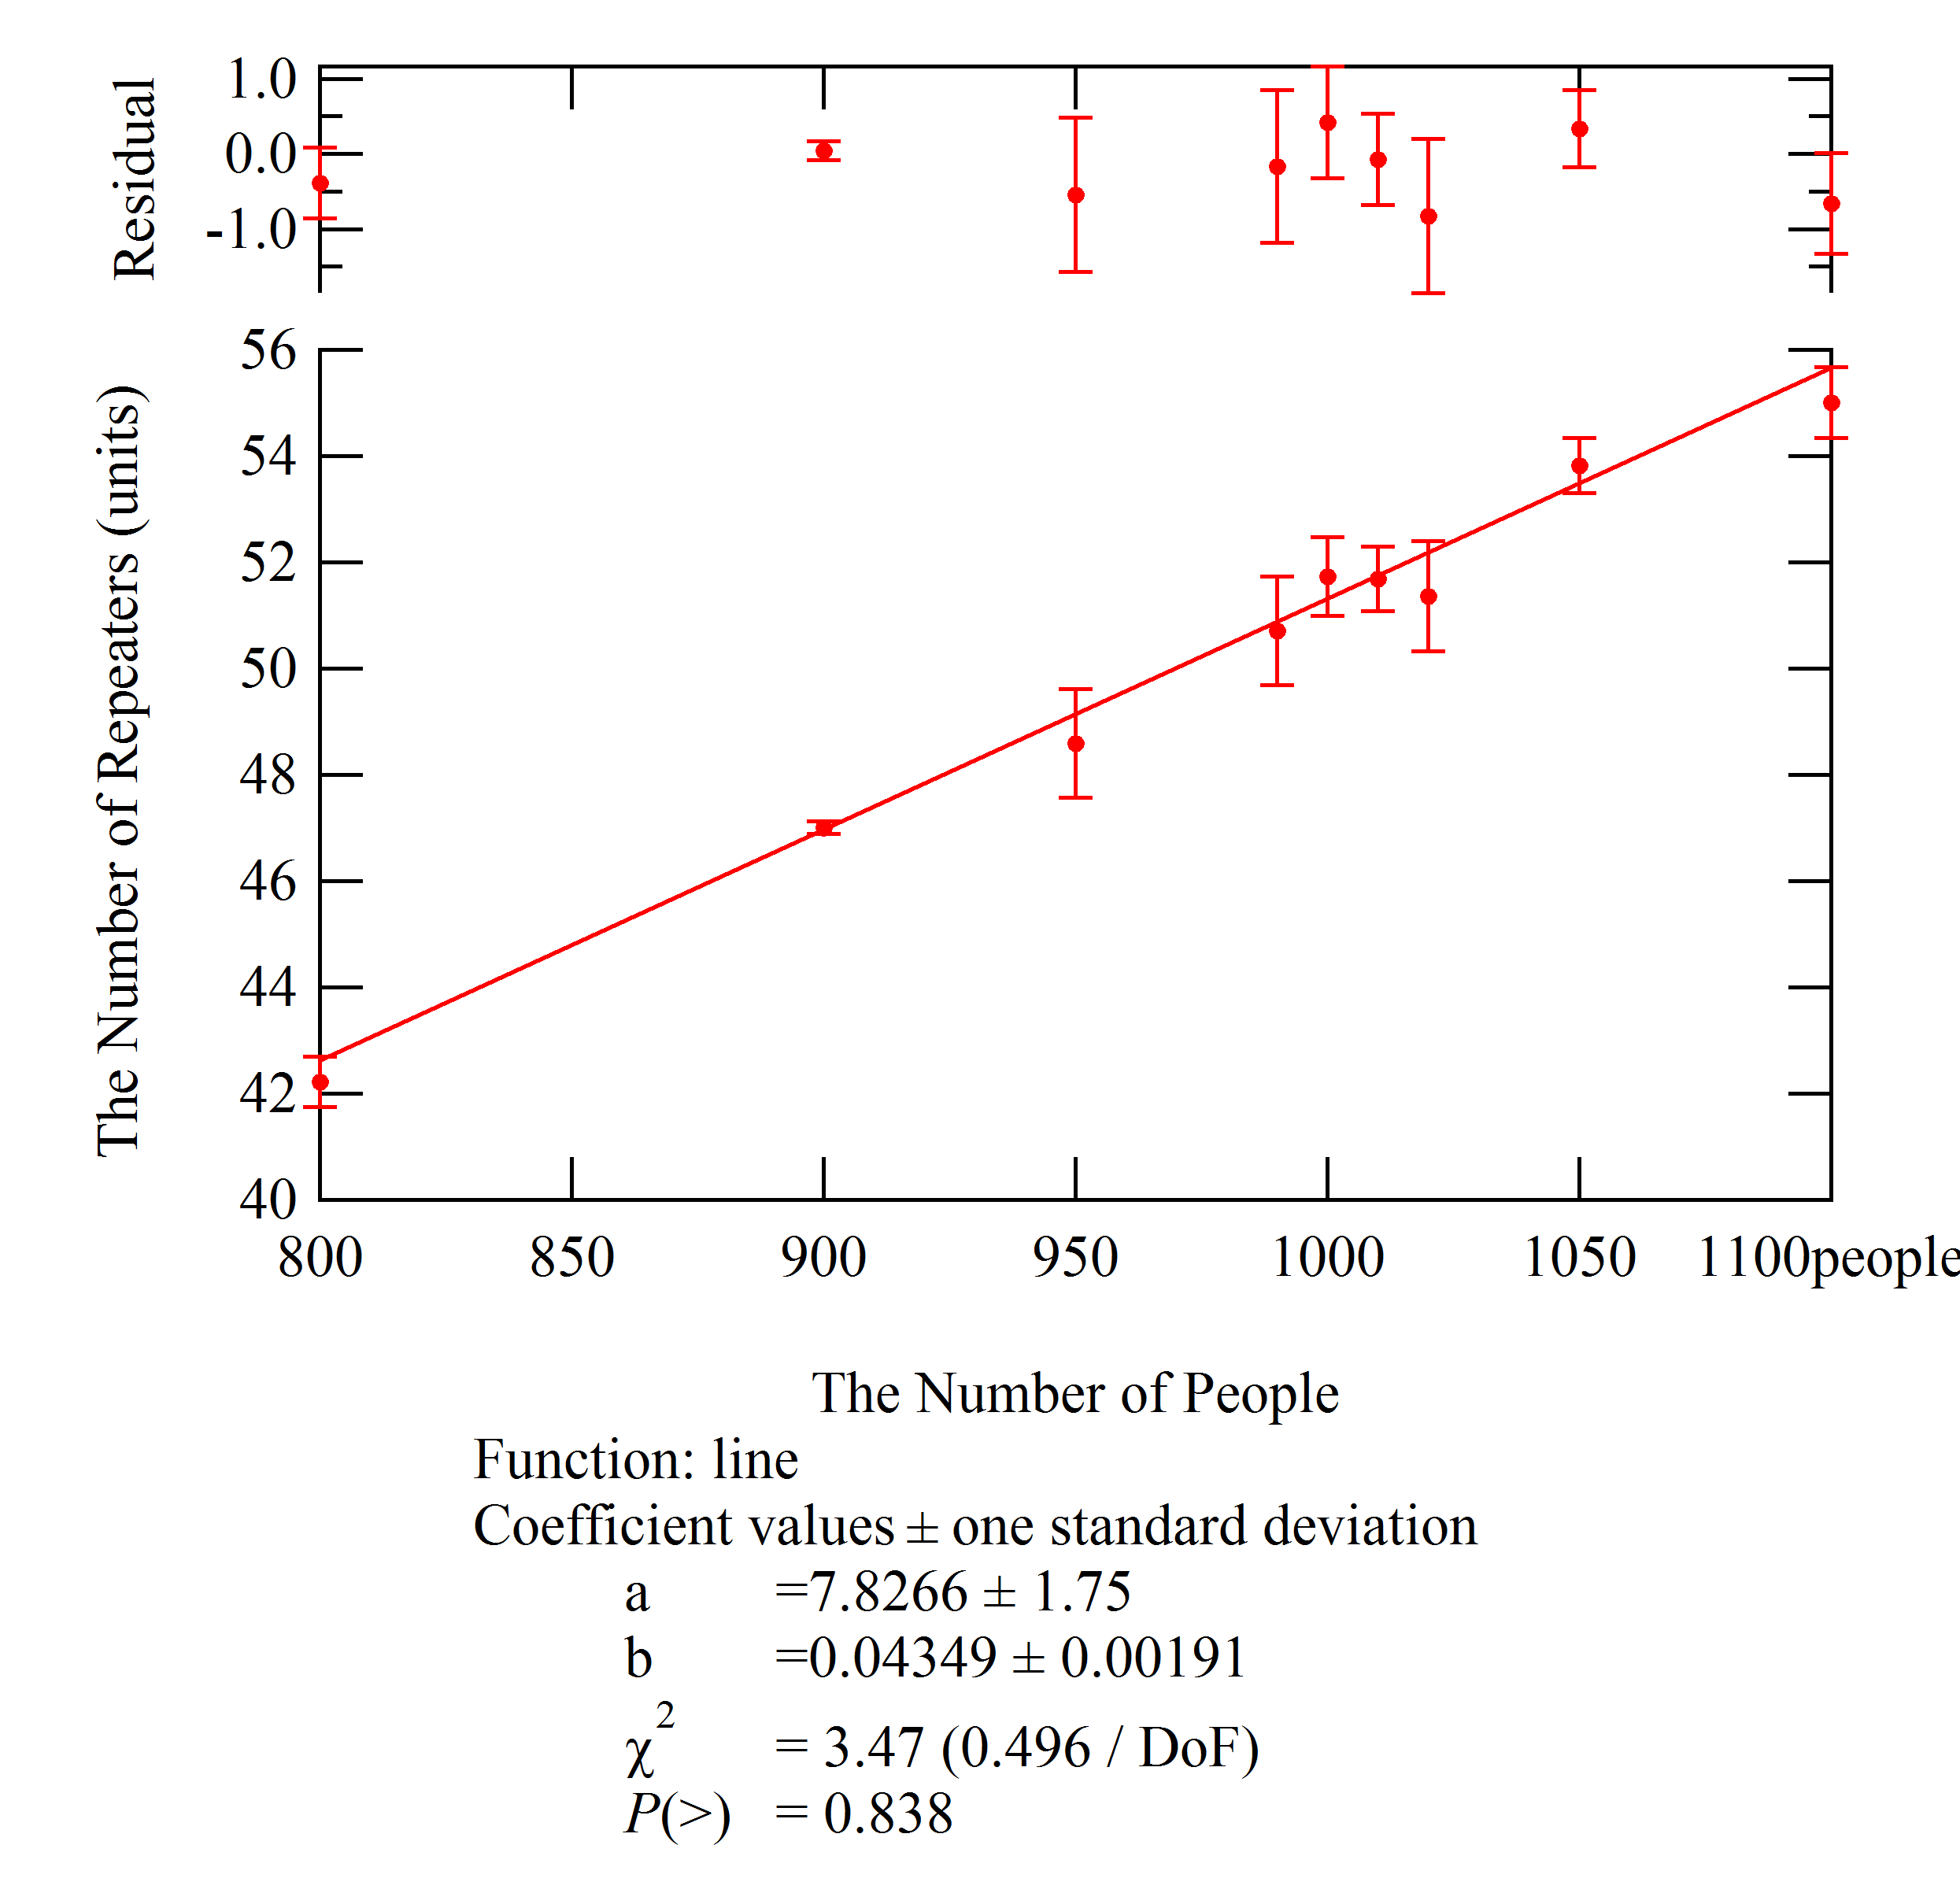
\includegraphics{sensitivity}}
\end{center}
\caption[Sensitivity of the Model]{Sensitivity Analysis with a Change in the Number of People.\label{sensitivity}}%
\label{fig:sensitivity}
\end{figure}
The reduced Chi-square value for this data set is 0.496. This is a good value, indicating that the number of repeaters is proportional to the number people, although the negative deviation this reduced Chi-square from 1.000 suggests that the line fits the data too well. The cause of this happening might be because we generate an almost completely randomized distribution of people. In the reaility, though, the distribution will be be as uniform as our model. For this particular data, the number of repeaters needed for 1,000 people is \boxed{51.7\pm 0.7 \text{ units.}}
\section{Comments}
Strength: accuracy of counting!
Weakness: need not be at the node.

\section{The Model Algorithm}
<<<<<<< HEAD
Explain it here.
=======
The algorithm works primarily by giving a different weight to each of the 
opics based on who is in the conversation. 
A conspirator is more likely to be discussing 
>>>>>>> 8014abb811481be1aae3700a703b0096d00c54f7

\section{Adapted Models}
\subsection{The population of 10,000 people}
In this case, I think the center of the town will have a lot of problems because we don't have enough PL tones and sets of frequencies to distinquish to coming signals. Our program reports the number of repeaters needed at the center as large as 1377, corresponding to the actual required number of repeaters of 514 with help of PL tones, and so each location needs approximately 10 sets of frequencies. We only have 3. There are many ways to solve this, such as extending the range of frequency, extending the area, and increasing the number of PL tones.

\subsection{Mountainous Area}
For the area that is mountainous, the range $R$ of each repeater is decreased. Therefore, we need more chains of repeaters in order to accomplish the same task. The level of haxagons will increase. If we set it to five, here is a result when we have 1,000 people:

Figure~\ref{mountainous} is an example of repeater coordination for a mountainous area.
\begin{figure}[ht]
\begin{center}
\scalebox{0.6}{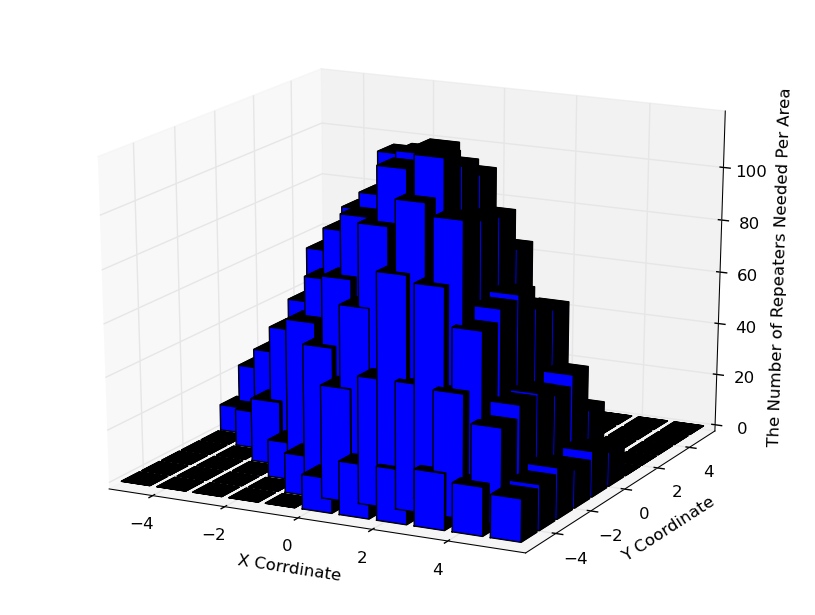
\includegraphics{mountainous}}
\end{center}
\caption[A Distribution of Repeaters for a Mountainous Area]{Distribution of Repeaters for a Mountainous Area (Maximum at the Middle).\label{mountainous}}
\label{fig:an-eps-graphic}
\end{figure}
Total is 4831.0. The repeaters per 1PL tone is  is 89.46 (This value reflects the total number of repeaters needed). Per one location is 0.596. We have 3 sets of frequencies, so this case will be easy to deal with. The peak at the middle is about 158.42. The number of sets of frequencies needed is 
$$\frac{158.42}{(\text{The number of areas})(\text{The number of PL tones})},$$
which is 
$$\frac{158.42}{(6\cdot 5^2)(54)}=\boxed {0.020.}$$
This value means that we can use only one frequency even at the middle of the town.  Although this data suggests that we need to use more repeaters (as much as 90 repeaters, as opposed to 52 repeaters), we perform better in terms of avoiding frequency interference.

\section{Possible Improvements}
\begin{enumerate}
\item Add the ability to adjust the number of people to do penalty: int(original/k), varying k.
\item Consider the bosses (Jerome, Delores, Gretchen) more carefully.
\item Keep the level of suspiciousness for 7, 11, 13 (or at least see how those change)
\item Implement semantic network analysis. 
	Or even now we notice some spanish stuff in more than one topic discussion
	so we can maybe group the topic or somehow tie the scores of those topics together
\item Think about the relationship to other fields: infected, diseased cells in a bio network
\end{enumerate}
		

\section{Conclusion}

All's well that ends well.


%%% ---------------
%%% Bibliography

%\nocite{*}   %%% Include everything in the thesis.bib file.  Be
             %%% careful---some journals and fields expect you to only
             %%% include references for materials that you have
             %%% actually cited in your paper, others allow you to
             %%% include materials you used as ``background'' without
             %%% actually citing specific pages or passages.

%%% Feel free to choose any bibliography style you like.
\bibliographystyle{plainnat}
%%% The filename (without the bib extension) of your bibliography file.
\bibliography{icmmcm}

\end{document}



